\chapter{Algoritmi euristici}\label{HEURISTIC}
In questo capitolo verranno trattati algoritmi euristici che non fanno uso di CPLEX. La necessità di non utilizzare CPLEX si ha per istanze con un elevato numero di nodi.\\
Per queste istanze la risoluzione del tableau attraverso CPLEX diventerebbe molto un'operazione molto onerosa per via dell'alto numero di variabili che verrano create e su cui verrà svolto il calcolo.\\
Attraverso gli algoritmi euristici, viene computata un'approssimazione della soluzione ottima e spesso però può essere sfruttata inizialmente dal risolutore CPLEX. Ad esempio questo può essere aggiunta prima della computazione, utilizzando la funzione \textit{CPXaddmipstarts()}, o ,se già definita, può essere modificata tramite \textit{CPXchgmipstarts()}.\\
Un algoritmo euristico, affinchè funzioni al meglio, deve essere composto da due fasi che si alternino:
\begin{itemize}
\item{\textbf{Intensificazione o raffinamento}\\
In questa fase la soluzione corrente viene migliorata fino al raggiungimento di un ottimo (locale o globale) nello spazio delle soluzioni.
}
\item{\textbf{Diversificazione}\\
Fase in cui la soluzione viene perturbata con una politica predefinita affinchè si allontani da un ottimo locale nello spazio delle soluzioni.
}
\end{itemize}


\section{Algoritmi di costruzione}\label{construction_alg}
Questa tipologia di algoritmi euristici è fondamentale per la computazione di una prima soluzione ammissibile del problema.
\subsection{Nearest Neighborhood}
Questo algoritmo è basato su un approccio di tipo greedy. L'algoritmo sceglie inizialmente un nodo generico tra quelli che compongono il grafo ed in seguito seleziona iterativamente degli archi del grafo, secondo il criterio enunciato nella seguente sezione.\\
In ciascuna iterazione vengono analizzati gli archi uscenti dal nodo selezionato all'iterazione precedente e viene aggiunto il ramo collega l'estremo più vicino. Il nuovo nodo raggiunto verrà impostato come punto di partenza nell'analisi dei costi dell'iterazione successiva (vedi Figura \ref{nearest_neighborhood}).
All'ultima iterazione viene selezionato invece l'arco che collega l'ultimo nodo visitato al nodo scelto randomicamente all'inizio dell'algoritmo.\\
Il problema di questo algoritmo è che in ogni iterazione viene selezionato esclusivamente il vertice più vicino a quello scelto precedentemente, senza però cercare di prevedere e migliorare la futura evoluzione del costo del tour, creato dall'algoritmo.\\
Come in Figura \ref{nearest_neighborhood}, la scelta dell'arco di costo minimo non implica che in seguito venga generata la soluzione ottima. La scelta del nodo iniziale è fondamentale in quanto una perturbazione della partenza genera un tour differente.\\
Definito \textbf{n} come il numero di nodi presenti nel grafo, si avranno quindi n soluzioni differenti, ottenute ciascuna attraverso l'applicazione dell'algoritmo partendo da una diversa scelta iniziale. In seguito tra queste possibli soluzioni, verrà selezionata quella di costo minore.\\
\begin{figure}[H] 
\begin{center} 
  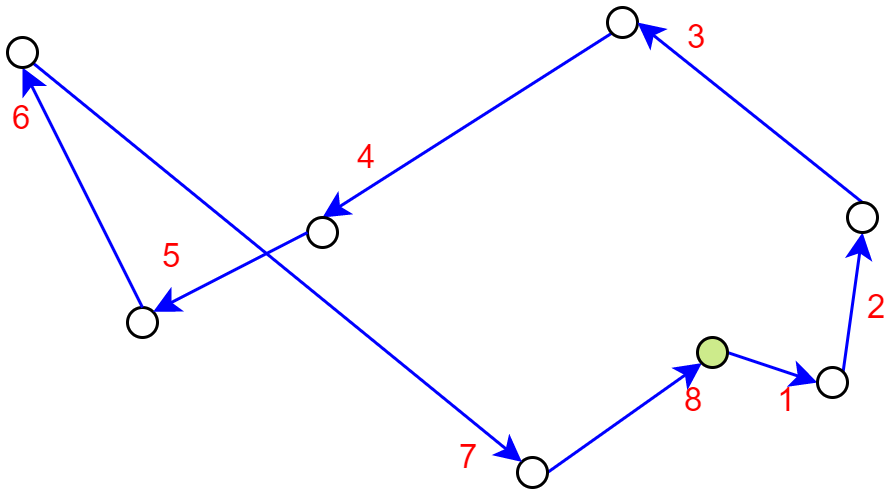
\includegraphics[scale=0.4]{Images/nearest_neighborhood}\\ 
  \caption{\footnotesize{Esempio di esecuzione di Nearest Neighborhood.}}
  \label{nearest_neighborhood} 
\end{center} 
\end{figure}

\subsection{Heuristic Insertion}
L'algoritmo seguente usa un approcco simile al precedente ma prevede inizialmente la selezione di un ciclo a cui apportare modifiche, per ottenere una soluzione iniziale ammissibile del problema. Per definire il ciclo di partenza vengono utilizzati diversi metodi. Di seguito sono riportati i due più utilizzati:
\begin{itemize}
\item{\textbf{Selezione di due nodi}\\
Vengono scelti i due nodi più lontani tra loro nel grafo, o due nodi casuali, e vegonono collegati mediante i due possibili archi orientati.
}
\item{\textbf{Inizializzazione geometrica}\\
Nel caso in cui i nodi del grafo appartengano ad uno spazio bidimensionale, ne viene calcolata la convex-hull e questa viene utilizzata come ciclo di partenza.
}
\end{itemize}
Questa prima soluzione viene modificata iterativamente e per ogni coppia di nodi non appartenenti al ciclo \textbf{C}, restituito dall'iterazione precedente, viene calcolato l'extramileage $\Delta_h$ come segue:
$$\Delta_h = \underset{(a,b)\in C}{min} c_{ah}+c_{hb}-c_{ay}$$
con $c_{ij}=$ costo dell'arco che collega i a j (vedi Figura \ref{partial_cycle}).\\
Alla fine di ciascuna iterazione viene aggiunto nel grafo il nodo \textbf{k} che minimizza l'\textbf{extra-mileage} (vedi Figura \ref{insertion}):\\
$$k = arg\underset{h}{min}\Delta_{h}$$
\begin{figure}[H] 
\begin{center} 
  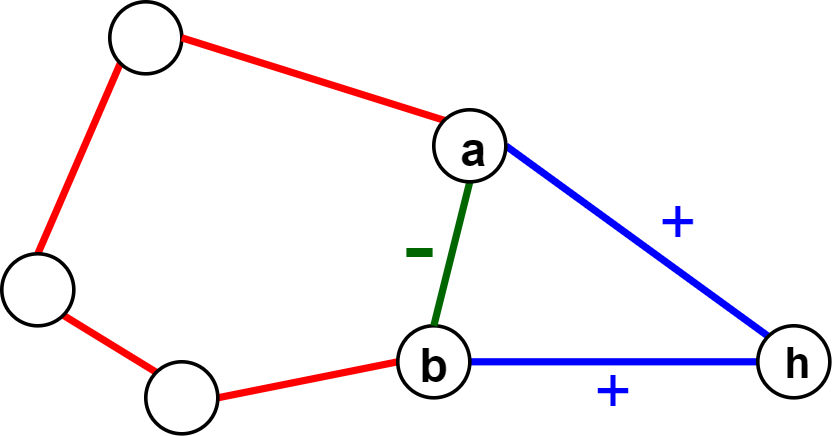
\includegraphics[scale=0.3]{Images/partial_cycle}\\ 
  \caption{\footnotesize{Parte del calcolo dell'extramileage del nodo \textbf{h}.}}
  \label{partial_cycle}
\end{center}
\end{figure}
\begin{figure}[H] 
\begin{center} 
  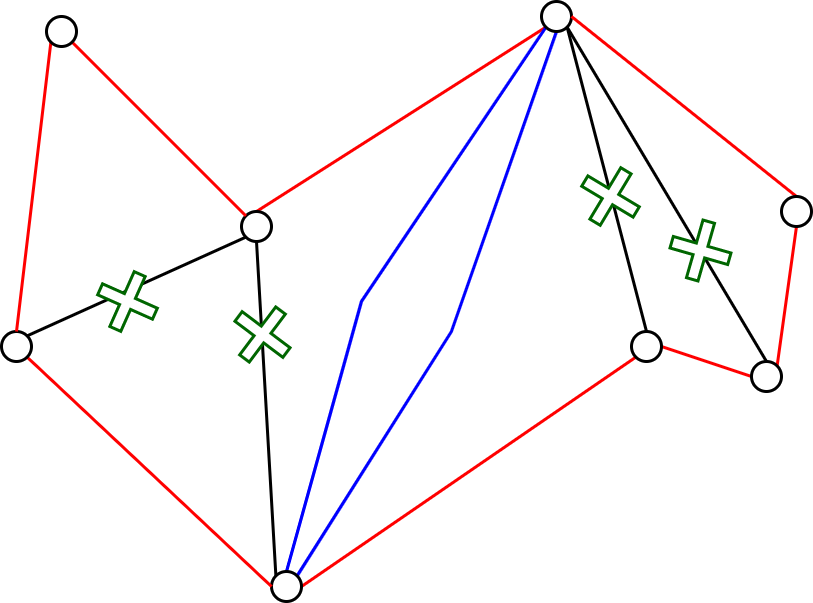
\includegraphics[scale=0.4]{Images/insertion}\\ 
  \caption{\footnotesize{Esempio dell'applicatione di Heuristic insertion.}}
  \label{insertion}
\end{center}
\end{figure}

\subsection{GRASP}
Il metodo Greedy Adaptive Search Procedure (GASP) è un approccio algoritmico che permette di aggiungere una componente aleatoria alla computazione deterministica del minimo di un insieme di valori.\\
Ad ogni iterazione dei due precedenti algoritmi di costruzione, invece di selezionare l'arco di costo minimo o l'extra-mileage minimo, vengono memorizzati i rami di costo minore e le scelte con extra-mileage minore.\\
Tra le possibili mosse salvate, ne viene scelta randomicamente una. Nel programma sviluppato, oltre ai precedenti algoritmi di costruzione, ne sono state impplementate anche delle varianti che fanno uso del GRASP. In questo caso sono state memorizzate le tre scelte migliori in ogni iterazione.\\
Tali varianti permettono di modificare aleatoriamente l'evoluzione del tour, in modo da evitare che, nelle ultime iterazioni dell'algoritmo, le scelte possibili siano legate esclusivamente ad elevati incrementi della funzione obiettivo.\\
Ciò evita ad esempio che nel Nearest Neighborhood possano esserci numerose scelte come l'ultima effettuata in Figura \ref{nearest_neighborhood}.\\
Nella Sezione \ref{Construction_perf}, vengono confrontati tramite performance profile, gli algoritmi precedentemente nominati.

\section{Algoritmi di raffinamento}
Una volta ottenuta una prima soluzione è necessario migliorarla per avvicinarsi il più possibile all'ottimo. Gli algoritmi utilizzati con questo scopo sono detti \textit{algoritmi di raffinamento}. Nel capitolo precedente sono già stati descritti due procedimenti di questo tipo, l'Hard Fixing e il Soft Fixing (vedi sottosezioni \ref{hard fixing} e \ref{soft fixing}). In questa sezione verranno invece analizzati algoritmi di raffinamento che non utilizzino funzioni messe a disposizione da CPLEX.

\subsection{Algoritmo di 2-ottimalità}
Nelle soluzioni restituite dagli algoritmi euristici di costruzione sono spesso presenti incroci tra coppie di rami. La loro presenza implica che la soluzione non è ottima, in quanto per le proprietà dei triangoli esisterà sempre una tour che eviti l'incrocio e che sia di costo minore (vedi Figura \ref{cross}). 
\begin{figure}[H] 
\begin{center} 
  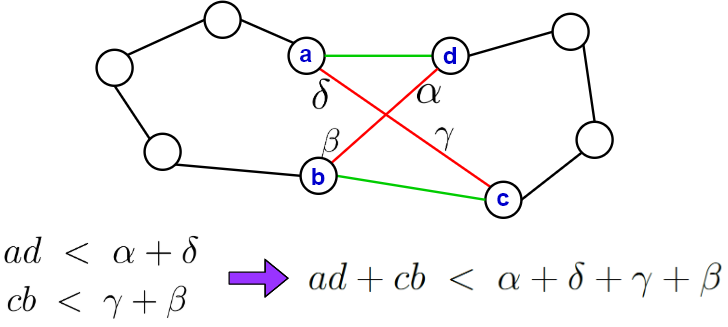
\includegraphics[scale=0.5]{Images/triangle_property}
  \caption{\footnotesize{Non ottimalità di una soluzione con incroci.}}
  \label{cross}
\end{center}
\end{figure}
L'algoritmo di 2-ottimilità prende il nome dalla modalità utilizzata iterativamente per modificare la soluzione ricevuta in ingresso. In ogni iterazione viene individuato un incrocio tra due rami, appartenenti al tour. Gli estremi di tali archi vengono collegati in maniera differente. Complessivamente per ogni incrocio, viene effettutato uno scambio tra coppie di rami (2-opt move) in modo da ridurre ulteriormente il costo della soluzione restituita.\\
Nell'implementare tale algoritmo non è necessario individuare ciascun incrocio della soluzione di partenza ma è sufficiente analizzare tutte le coppie di rami presenti e verificare se, scambiandole con un'altra coppia ammissibile, si verifichi un miglioramento della funzione obiettivo.
\begin{figure}[H] 
\begin{center} 
  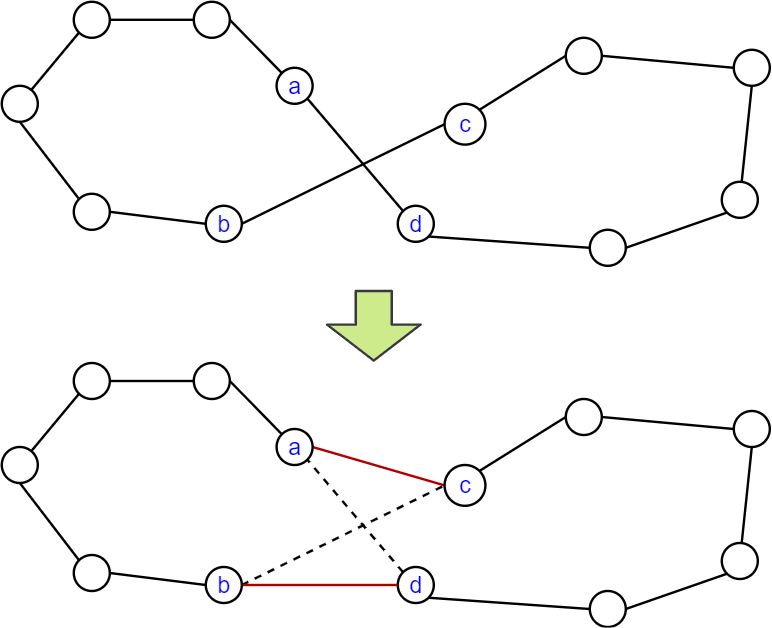
\includegraphics[scale=0.4]{Images/swap}\\ 
  \caption{\footnotesize{Esempio di eliminazione di un incrocio.}}
  \label{swap}
\end{center}
\end{figure}
Riferendosi alla figura \ref{swap}, un possibile miglioramento viene calcolato come segue:\\
$$\Delta = (c_{ac} + c_{bd}) - (c_{ad} + c_{bc})$$
e solo nel caso in cui $\Delta$ sia negativo, la sostituzione viene effettuata.\\
Applicando una 2-opt move al circuito attuale, viene generato un tour appartenente all'intorno di 2-ottimalità della precedente soluzione. Ripetendo iterativamente tale procedimento si raggiunge un ottimo locale, in cui non esistono più possibili miglioramenti della funzione obiettivo. Questo processo è rappresentato in Figura \ref{two_optimality}. 
\begin{figure}[H] 
\begin{center} 
  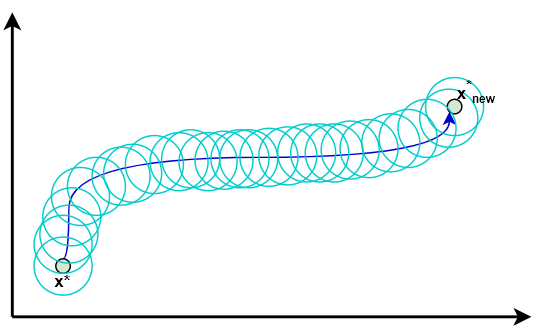
\includegraphics[scale=0.4]{Images/two_optimality}\\ 
  \caption{\footnotesize{Aggiornamento della soluzione nell'intorno di 2 ottimalità.}}
  \label{two_optimality}
\end{center}
\end{figure}
Poichè il calcolo del $\Delta$ avviene in tempo costante e deve essere fatto per ogni coppia di rami, il tempo complessivo per la computazione è $O(n^2)$, con $n$ nodi dell'istanza del problema.\\
Un procedimento analogo a tale algoritmo viene utilizzato anche nel Soft Fixing, in cui però la dimensione dell'intorno in cui cercare la nuova soluzione varia (vedi Figura \ref{local_exe}).\\
Nel programma sviluppato, è stata utilizzata questo algoritmo per rimuovere gli incroci all'interno del tour.
 
\subsection{Algoritmo di 3 ottimalità}
L'algoritmo di 3 ottimalità è analogo a quello analizzato nella sezione precedente, ma considera intorni di grandezza maggiore. In questo caso, quindi, due soluzioni nell'intorno differiscono per 3 rami. In Figura \ref{three_optimality} viene riportata la rappresentazione delle possibili 3-opt move.
\begin{figure}[H] 
\begin{center} 
  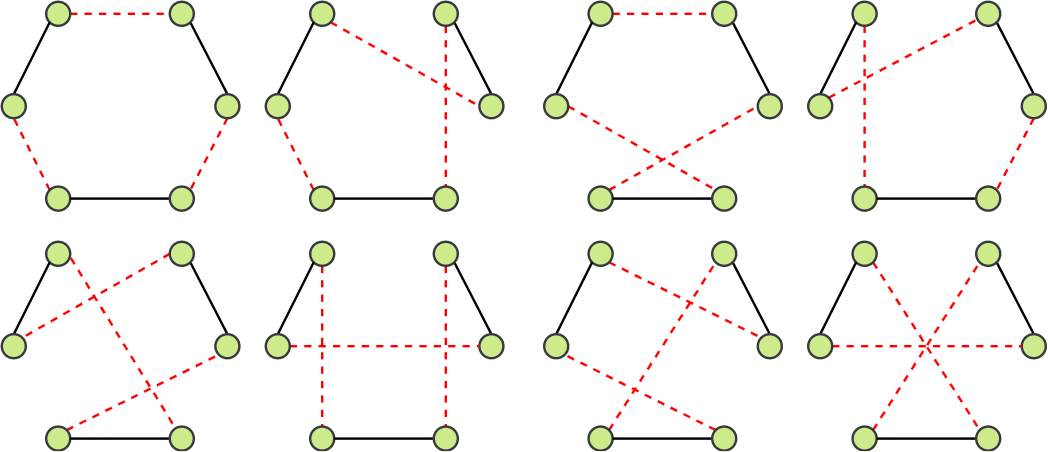
\includegraphics[scale=0.35]{Images/3_swap}
  \caption{\footnotesize{Tutte le possibili combinazioni di scambi di 3 ottimalità.}}
  \label{three_optimality}
\end{center}
\end{figure}
L'algoritmo impiega in tutto $O(n^3)$ (con $n$ numero di nodi) per trovare un ottimo locale, essendo $O(n^3)$ il numero di terne di rami esistenti e poichè il numero di possibili scambi di 3 ottimalità è costante. Su istanze con un elevato numero di nodi, il tempo di calcolo risulterebbe essere troppo lungo per il calcolo di una soluzione.\\
All'interno del programma sviluppato, non è stata implementato tale algoritmo.

\section{Meta-euristici}
Gli algoritmi di raffinamento appena visti si occupano di migliorare il più possibile una soluzione già calcolata attraverso meccanismi di local search. In questo modo, dopo un determinato numero di iterazioni, viene raggiunto un ottimo locale.\\
Gli algoritmi descritti in questa sezione perturbano la soluzione allontanandola dall'attuale ottimo locale e cercando di avvicinarsi il più possibile all'ottimo globale.\\
Questi metodi rappresentano approcci più generali di quelli descritti precedentemente e sono plasmabili e applicabili anche a problemi differenti rispetto al TSP. Tali tecniche infatti permettono essenzialmente di esplorare lo spazio delle soluzioni, evitando di stazionare in minimi o massimi locali con valori della funzione obiettivo molto lontani dall'ottimo globale.

\subsection{Multi-start}
Un primo e intuitivo approccio per allontanarsi da un ottimo locale è quello descritto dalla politica multi-start. Questa consiste nel definire diverse soluzioni attraverso un algoritmo di costruzione tra quelli descritti, ad esempio, nella Sezione \ref{construction_alg}.\\
A ciascuno di esse viene poi applicato un algoritmo di raffinazione e viene scelta solo quella con costo migliore tra tutte le soluzioni generate. In questo modo vengono analizzati diversi ottimi locali nello spazio delle soluzioni (vedi Figura \ref{multi_start}. 
\begin{figure}[H] 
\begin{center} 
  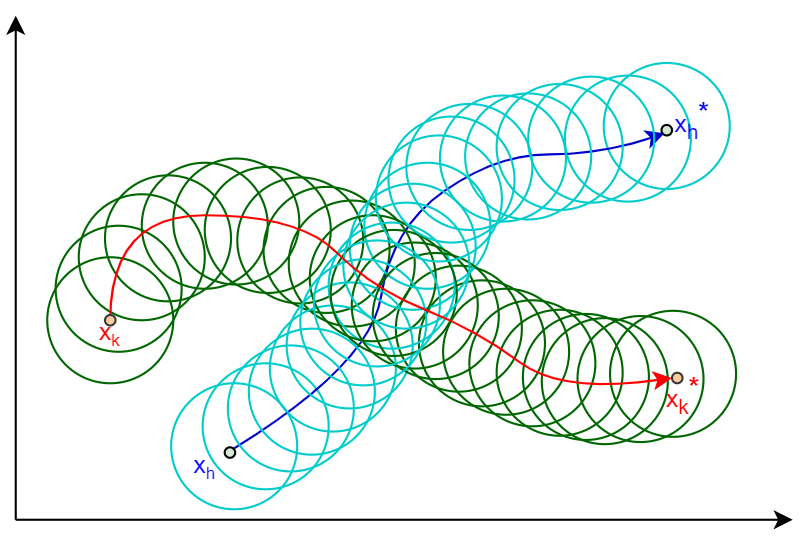
\includegraphics[scale=0.5]{Images/multistart}\\ 
  \caption{\footnotesize{Due possibile esecuzioni di un algoritmo di raffinamento con partenze da due soluzioni diverse.}}
  \label{multi_start}
\end{center}
\end{figure}
Un lato negativo di tale approccio consiste nel fatto che ogni volta che viene scelta una nuova soluzione di partenza, vengono perse le informazioni relative alla sequenza ottenuta utilizzando un altro tour iniziale. La soluzione implementata all'interno del programma è basata sul multithreading. Infatti viene generato un numero di soluzioni pari al numero di thread specificati.\\
Ciascun thread genera parallelamente agli altri una nuova soluzione e solo al termine della computazione, la confronta con la migliore. Nel caso in cui il costo della soluzione trovata sia inferiore a questa, la aggiorna. \\
Nella Sezione \ref{construction_perf} viene analizzato il costo ottenuto dalla nostra implementazione, utilizzando 12 thread e modificando l'algoritmo di costruzione utilizzato.

\subsection{Variable Neighborhood Search}
Il Variable Neighborhood Search (VNS) è un algoritmo che cerca di migliorare l'ottimo locale attuale, ricevuto in input, analizzando intorni di ottimalità di grandezza differente.\\
Nel caso in cui non si trovi una nuova soluzione, di costo migliore di quella attuale nei vari intorni di grandezza k, l'algoritmo prevede che venga scelto un certo numero di rami in maniera randomica da sostituire con altri archi\cite{VNS}. In questo modo si impone un aggiornamento peggiorativo in termini di costo, nella speranza che nel nuovo intorno selezionato sia possibile trovare una soluzione che si allontani dall'ottimo locale di partenza (vedi Figura \ref{VNS_img}).\\
 \begin{figure}[H] 
\begin{center} 
  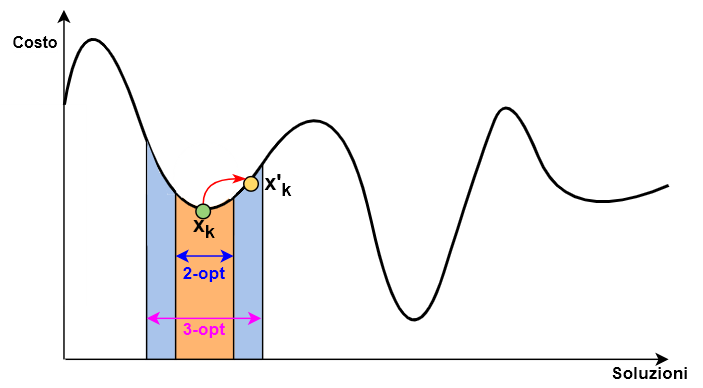
\includegraphics[scale=0.4]{Images/VNS}\\ 
  \caption{\footnotesize{Aggiornamento di una soluzione in un minimo locale.}}
  \label{VNS_img}
\end{center}
\end{figure}
L'algoritmo termina allo scadere di una deadline, inserita dall'utente, o dopo un determinato numero di iterazioni, restituendo la miglior soluzione trovata fino a quell'istante. Utilizzando questo approccio gran parte della soluzione di partenza viene conservata evitando di perdere le informazioni elaborate precedentemente eseguendo l'algoritmo.\\
La nostra implementazione dell'algoritmo VNS non è però quella classica ma una variante detta VNS ibrido\cite{hybrid_VNS}. Di seguito viene descritto lo pseudo-codice di tale metodo:\\\\
\begin{algorithm}[H]
\DontPrintSemicolon
\KwIn {$\mathtt{x =\{x_1,x_2,...,x_n\}}$= sequenza di visita dei nodi nella soluzione di partenza (ottimo locale)\newline}
\KwOut {$\mathtt{y}$= nuova soluzione appertenente all'intorno di k-ottimalità di x}
\BlankLine
\While{$'deadline\;not\;expired'$ $\wedge$ $count<MAX\_COUNT$}{
\BlankLine
$\mathtt{y\gets} x$\;
$\mathtt{k\gets}1$\;
\BlankLine
 \While{$k\leq \lceil n/2 \rceil$}{
  \BlankLine
  $N_k(y) = \{ (y_1,...,y_{(i+k)mod\;n},...,y_i, ..., y_n)\; :\; 1\leq i\leq n\}$\;
  \BlankLine
  \If{$\underset{z\in N_k(y)}{min}\{cost(z)\}<cost(x)$}{
	 $\mathtt{x\gets} \underset{z\in N_k(y)}{argmin(cost(z)}$\;
     $\mathtt{y\gets} \underset{z\in N_k(y)}{argmin(cost(z)}$\;
	 $\mathtt{break}$\;
     \BlankLine
  }
  \BlankLine
  $\mathtt{k}\gets k+1$\;
  \BlankLine
 }
 \If{$k>\lceil n/2 \rceil$ $\wedge$ $!found$}{
    \BlankLine
    $\mathtt{y}\gets \mathtt{new\_random\_sol(} y \mathtt{)}$\;
    \BlankLine
 }
  $\mathtt{count}\gets count+1$\;
}
 \caption{VNS ibrido}
\end{algorithm}
Partendo dalla sequenza di visita dei nodi nella soluzione locale, passata in ingresso all'algoritmo, la procedura analizza tutte i circuiti ottenuti invertendo due nodi a distanza k nella sequenza, con $k=1,...,n/2$. Se viene individuata una soluzione con costo inferiore, allora questa viene considerata come il nuovo ottimo locale. Invece se non dovesse esistere alcuno scambio migliorativo, viene scelta in maniera randomica una nuova soluzione dall'insieme:
$$\biggl\{{y}\cup \bigcup_{k=1}^{\lceil n/2 \rceil}{N_k(y)}\biggr\}$$
con probabilità pari a:
$$p=\frac{costo^{-1}(x)}{\underset{z \in {\bigcup_{k=1}^{\lceil n/2 \rceil}{N_k(y)}}}\sum{costo^{-1}(z)}}$$
Nell'implementazione sono state sviluppate due versioni di questo algoritmo, in base alle probabilità utilizzata nel selezionare due nodi da scambiare: 
\begin{itemize}
\item{\textbf{Hybrid VNS}\\
questa prima soluzione segue la procedura precedentemente descritta e seleziona una nuova sequenza dall'insieme $\{{y}\cup \bigcup_{k=1}^{\lceil n/2 \rceil}{N_k(y)}\}$ e poi vi applica un algoritmo di raffinamento.} 
\item{\textbf{Hybrid VNS Uniform}\\
questa variante invece seleziona due nodi della sequenza di visita, secondo una probabilità uniforme, e li scambia. La sequenza risultante, dopo essere stata migliorata mediante un algoritmo di raffinamento, viene utilizzata come nuovo minimo locale.}
\end{itemize}
la prima che seleziona uno scambio secondo questa probabilità, e la seconda che invece seleziona due elementi casuali della sequenza e li scambi secondo una distribuzione uniforme.

\subsection{Tabu Search}
Il metodo Tabu Search fu ideato da Fred W. Glover \cite{Tabu}. Dato un ottimo locale nello spazio delle soluzioni, l'idea di Glover permette di aggiornarla anche con una di costo più elevato, cercando di minimizzarlo. Per evitare che all'iterazione successiva si ritorni nella soluzione di partenza, viene creata una lista di "mosse vietate", detta Tabu List, che impedisca di raggiungere nuovamente lo stesso ottimo locale. In questo modo il costo della soluzione attuale aumenta rispetto all'ottimo locale di partenza per un certo numero di iterazioni, finchè non ricominci a decrescere per raggiungere un nuovo minimo. Nella nostra implementazione la lista viene riempita con i rami che vengono rimossi per creare la nuova soluzione.\\
Aumentando costantemente di dimensione la lista Tabu si rischia, ad un certo punto, che non sia più possibile modificare il tour presente. Per evitare ciò generalmente viene scelta una capienza massima, detta \textit{tenure}, della lista, una volta raggiunta i rami vengono aggiunti rispettando la politica FIFO (first in first out).\\
Per aumentare le prestazioni dell'algoritmo è possibile far variare le dimensioni della Tabu List tra due valori. Nella fase di diversificazione la lista viene fatta aumentare fino ad un massimo (nella nostra implementazione 1/5 del numero di nodi dell'istanza da risolvere). Nella fase di intensificazione, per lasciare un maggior numero di gradi di libertà al definizione delle nuove soluzioni, la tenure diminuisce fino ad un valore minimo impostato, che nel nostro caso corrisponde a 1/10 del numero di nodi del grafo (vedi Figura \ref{tenure}). Questo variante dell'algoritmo, implementata anche nel nostro programma, in letteratura è conosciuta con il nome di \textit{Reactive Tabu Search}.
 \begin{figure}[H] 
\begin{center} 
  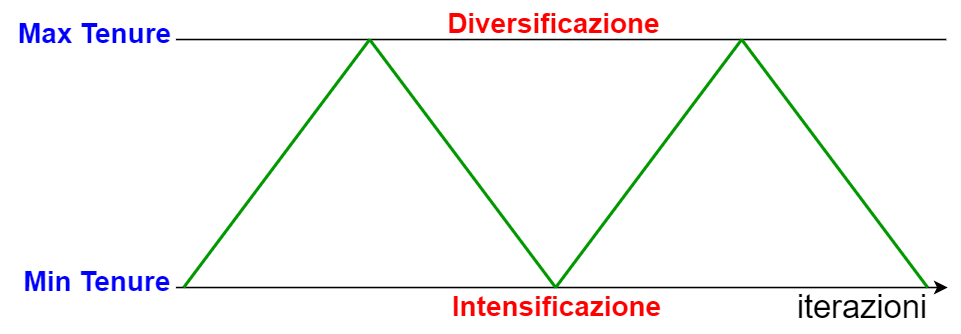
\includegraphics[scale=0.35]{Images/tenure}\\ 
  \caption{\footnotesize{Variazione della tenure.}}
  \label{tenure}
\end{center}
\end{figure}
Come per l'algoritmo precedente, il criterio di terminazione è dato dallo scadere del tempo a disposizione o dal raggiungimento di un numero massimo di iterazioni. La soluzione restituita dall'algoritmo è la migliore individuata  fino a quell'istante.\\\\
\begin{algorithm}[H]
\DontPrintSemicolon
\KwIn{$\mathtt{x}$= soluzione di un'istanza di TSP corrispondente ad un ottimo locale\newline
$\mathtt{tenure}$= dimensione massima della Tabu List\newline
$\mathtt{deadline}$= time limit complessivo dell'algoritmo\newline
$\mathtt{num\_iterations}$= numero massimo di iterazioni\newline
$\mathtt{num\_nodi}$= numero di nodi dell'istanza tsp\newline}
\KwOut {$\mathtt{y}$= miglior soluzione trovata}
\BlankLine
$\mathtt{n}=0$\;
\BlankLine
\While{$n < num\_iterations \wedge\;\;'deadline\;not\;expired'$}{
 \BlankLine
 $\mathtt{x' \gets move\_random\_2opt(}x)$\;
 \BlankLine
 \BlankLine
\While{$(check\_tabu\_list(x') ==\;'valid\;move')$}{
  \BlankLine
  $\mathtt{x' \gets move\_random\_2opt(}x\mathtt{)}$\;
}
  $\mathtt{x} \gets x'$\;
  $\mathtt{add\_tabu\_list(}edges\_removed, tenure\mathtt{)}$\;
  \BlankLine
  \If{$cost(x') < cost(x)$}{
    \BlankLine
    $\mathtt{x \gets greedy\_refinement(}x, tabu\_list\mathtt{)}$\;
    \BlankLine  
  }
  \BlankLine
  $\mathtt{n \gets}n+1$\;
}
 \BlankLine
$\mathtt{y}= best\_solution()$\;
\caption{Tabu Search}
\end{algorithm}
\subsection{Simulated annealing}
L'algoritmo Simulated Annealing, come dice il nome, è ispirato al processo di temperamento dei metalli, in cui un materiale viene raffreddato molto lentamente e in maniera controllata, affinché raggiunga la configurazione di minima energia. Analogamente, nell'algoritmo viene scelta una funzione (generalmente esponenziale) che simula la variazione della "temperatura" $T$. Nella nostra implementazione abbiamo utilizzato la seguente formula \cite{SA}:
$$T = \alpha^{num\_iteration}* T\_max \;+\; T\_min$$
dove \textit{T\_max} è la massima temperatura iniziale, \textit{T\_min} è la minima temperatura che può essere raggiunta, \textit{num\_iteration} è il numero di iterazioni eseguite fino a quel momento e \textit{$\alpha$} è un parametro scelto all'inizio dell'esecuzione. Nello sviluppare questo procedimento sono stati utilizzati i seguenti valori:
\begin{itemize}
\begin{multicols}{3}
\item{\textit{T\_max} = 5000}
\item{\textit{T\_min} = 100}
\item{\textit{$\alpha$} = 0.99}
\end{multicols}
\end{itemize}
Una volta raggiunta la temperatura minima, nel caso in cui non sia scaduto il tempo a disposizione, $T$ viene impostata nuovamente a \textit{T\_max}, per poter procedere con la computazione.\\ 
 Ad ogni iterazione la soluzione corrente può essere aggiornata con un'altra qualsiasi  interna all'intorno di 2 ottimalità, di costo minore o maggiore, con una probabilità funzione della variazioni di costo e della temperatura attuale, $f(\Delta costo, T)$. Nel nostro caso la seguente\cite{SA}:
$$P = 
\begin{cases}
1 & se\; \Delta costo \leq \;0\\
exp(- \frac{\Delta costo}{T}) & se\; \Delta costo \;>\;0\\
\end{cases}
$$
Grazie a questa tecnica per la scelta dell'aggiornamento, non è necessario scandire tutto l'intorno, è sufficiente scegliere in maniera randomica 2 rami. Tali archi verranno sostituiti nella soluzione corrente secondo la funzione di probabilità (Figura \ref{simulated_annealing}).
 Per poter gestire al meglio i valori della probabilità e evitare che la maggior parte delle volte venissero approssimati a zero, nel nostro algoritmo sono stati riscritti in notazione scientifica, memorizzando solo l'ordine di grandezza e il coefficiente. Una nuova soluzione di costo peggiore viene, quindi, accettata nel caso in cui si verifichino entrambe le seguenti situazioni 
\begin{itemize}
\item{venga estratto per un numero di volte pari all'ordine di grandezza, un numero, nell'intervallo [0, 99], inferiore a 10;}
\item{venga estratto, nell'intervallo [0, 10*(coefficiente della probabilità)], un numero inferiore a 10.}
\end{itemize} 
 \begin{figure}[H]
\begin{center} 
  \includegraphics[scale=0.43]{Images/simulated_anneling}
  \caption{\footnotesize{Esempio di esecuzione dell'algoritmo Simulated Annealing.}}
  \label{simulated_annealing}
\end{center}
\end{figure}
 Con il procedere delle iterazioni, l'aggiornamento ad un costo peggiore avviene sempre meno frequentemente, fino ad ottenere solo aggiornamenti con soluzioni più vantaggiose. Esiste un teorema secondo il quale se la temperatura varia in maniera estremamente lenta ed è consentito effettuare un numero di iterazioni estremamente elevato, questo algoritmo garantisce di trovare l'ottimo globale. Concretamente queste ipotesi sono molto difficili da realizzare, ma è statisticamente comunque possibile dichiarare che l'approccio del Simulated Annealing restituisce una buona soluzione.
 \begin{algorithm}[H]
\DontPrintSemicolon
\KwIn{$\mathtt{x}$=soluzione di un'istanza di TSP corrispondente ad un ottimo locale\newline
$\mathtt{T_{min}}$=temperatura minima\newline
$\mathtt{T_{max}}$=temperatura massima\newline
$\mathtt{deadline}$=time limit complessivo dell'algoritmo\newline
}
\KwOut {$\mathtt{y}$= miglior soluzione trovata}
\BlankLine
$\mathtt{T} \gets T_{min}$\;
\BlankLine
\While{$'deadline\;not\;expired'$}{
$\mathtt{x' \gets move\_random\_2opt(}x\mathtt{)}$\;
\BlankLine
\If{$cost(x') < cost(x)$}{
  $\mathtt{x'} \gets x$\;
  $\mathtt{update\_cost()}$\;
  }
  \BlankLine
\Else{
	$\mathtt{compute\_prob(}cost(x'), T\mathtt{)}$\;
	\BlankLine
	\If{$\mathtt{accepted(}x'\mathtt{)}$}{
		 $\mathtt{x'} \gets x$\;
 		 $\mathtt{update\_cost()}$\;
 		 $\mathtt{update\_temperature(}T\mathtt{)}$\;
	} 
  }
}
 \BlankLine
$\mathtt{y}= best\_solution()$\;
\caption{Simulated Annealing}
\end{algorithm}
\subsection{Algoritmo genetico}
L'algoritmo genetico è legato alla teoria dell'evoluzione di Darwin, con cui condivide numerosi concetti. Da un punto di vista teorico, l'algoritmo costruisce in prima battuta una serie di individui, che costituiscono una popolazione.\\
In seguito, attraverso mutazioni dei singoli soggetti e la riproduzione di questi, viene creata una nuova popolazione. Il concetto fondamentale alla base di tale algoritmo è che associando ad un individuo uno punteggio, detto fitness, lo si possa selezionare con una certà probabilità per far evolvere la specie.\\
Applicando tale concetto al Travelling Salesman Problem, ad ogni individuo $i$ viene associata una fitness pari a:
$$fitness_i=\frac{1}{costo_i}$$
dove $costo_i$ rappresenta il valore della funzione obiettivo per l'istanza $i$.\\
La popolazione iniziale è stata generata utilizzando l'algoritmo nearest neighbour ma utilizzando un diverso nodo di partenza per ciascuno di essi ed applicando anche la variante GRASP. Ogni individuo della popolazione è stato poi rappresentato come la sequenza di visita dei nodi della corrispondente soluzione.\\
In fase di testing, abbiamo notato che la creazione della popolazione costituisca il vero collo di bottiglia dell'intero algoritmo.\\
Per ridurre al minimo il carico computazionale di tale fase, questa è stata implementata in multithreading. I risultati sono complessivamente migliorati, anche se questa fase resta ancora un'operazione molto costoso in termini di tempo di calcolo.
In seguito la fase di evoluzione della popolazione viene effettuata generando nuovi individui a partire dalla popolazione attuale ed utilizzando le seguenti tecniche:
\begin{itemize}
\item{\textbf{Crossover}\\
in questa operazione vengono selezionati randomicamente due individui della popolazione e a partire da questi, vengono creati nuovi tour che ereditano dai genitori delle caratteristiche. Nel nostro caso ciascun nuovo individuo eredita metà della sequenza di visita da uno dei suoi genitori, e la restante parte viene ereditata dall'altro.}
\item{\textbf{Mutazione}\\
in questa fase un certo numero di individui viene selezionato in maniera casuale e da ciascuno di questi, viene generato un nuovo tour attraverso una sua permutazione casuale.}
\end{itemize}
Utilizzando iterativamente tali tecniche e rimuovendo gli individui di costo peggiore dalla popolazione, si riduce complessivamente il costo medio delle istanze nella popolazione e di conseguenza anche il costo della migliore soluzione. All'interno del programma sviluppato, le precedenti tecniche non sono state applicate contemporaneamente in ogni iterazione ma in istanti differenti, secondo quanto descritto nel seguente algoritmo.\\

\begin{algorithm}[H]
\DontPrintSemicolon
\KwIn {$\mathtt{population}$= popolazione di numerosi tour generati mediante un algoritmo di costruzione\newline}
\KwOut {$\mathtt{y}$= sequenza di visita dei nodi nel tour ottenuto di costo minore}
\BlankLine
 $\mathtt{num\_epochs} \gets$ 0\;
 $\mathtt{best\_cost} \gets$ 0\;
 \BlankLine
 \While{$\mathtt{num\_epochs} < MAX\_NUM\_EPOCHS$}{
  \BlankLine  
  \If{$num\_epochs\;mod\;3 == 0$}{
     \BlankLine    
     $\mathtt{crossover(}population, best\_cost\mathtt{)}$\;
  }
  \Else{
     \BlankLine    
     $\mathtt{mutation(}population, best\_cost\mathtt{)}$\;
  }
  \BlankLine
  $\mathtt{remove\_worst\_members(}population{)}$\;
  \BlankLine
 }
 
 $\mathtt{y}\gets best_member(population)$
 \caption{Evoluzione}
\end{algorithm}
La fase di crossover viene applicata più di rado, poichè la generazione di nuovi figli a partire dai genitori richiede molto più tempo della creazione dello stesso numero di individui mediante mutazione.\\
Gli algoritmi di crossover e mutazione, utilizzati nel programma sviluppato, sono descritti e illustrati di seguito.\\\\
\begin{algorithm}[H]
\DontPrintSemicolon
\KwIn {$\mathtt{population}$= popolazione di numerosi tour generati mediante un algoritmo di costruzione\newline
$\mathtt{sum\_fitnesses}$= somma delle fitness di tutti gli individui della popolazione \newline
$\mathtt{best\_cost}$= costo della migliore soluzione attuale\newline}
\KwOut {$\mathtt{offspring_1, offspring_2}$= nuovi individui generati nella popolazione\newline}
\BlankLine 
$\mathtt{n}$= numero di nodi dell'istanza tsp\;
$\mathtt{x=\{x_1,...,x_n\} \gets RANDOM(}population, p=\frac{fitness_x}{sum\_fitnesses})$\;
$\mathtt{y=\{y_1,...,y_n\} \gets RANDOM(}population, p=\frac{fitness_y}{sum\_fitnesses})$\;
 \BlankLine \BlankLine
 $\mathtt{offspring_1[1,...n/2]}=x[1,..., n/2]$\;
 $\mathtt{offspring_2[n/2+1,...,n]}=y[n/2+1,..., n]$\;
 $\mathtt{offspring_1[n/2+1,...,n]}=\{y_i\in y\; :\; y_i\not\in\{x_1, ..., x_{n/2}\}\}$\;
 $\mathtt{offspring_2[n/2+1,...,n]}=\{x_i\in x\; :\; x_i\not\in\{y_{n/2+1}, ..., y_{n}\}\}$\;
  \BlankLine
  $\mathtt{sum\_fitnesses\gets update(}sum\_fitness, offspring_1, offspring_2\mathtt{)}$\;
  \BlankLine  
  $\mathtt{min\_cost \gets min(}cost(offspring_1), cost(offspring_2)\mathtt{)}$\;  
  \BlankLine
  \If{$cost(offspring1) < best\_cost$}{
 	 $\mathtt{best\_cost} \gets min\_cost$\;
     \BlankLine
  }
\caption{Crossover}\label{crossover_pseudo}
\end{algorithm}

\begin{figure}[H]
\begin{center} 
  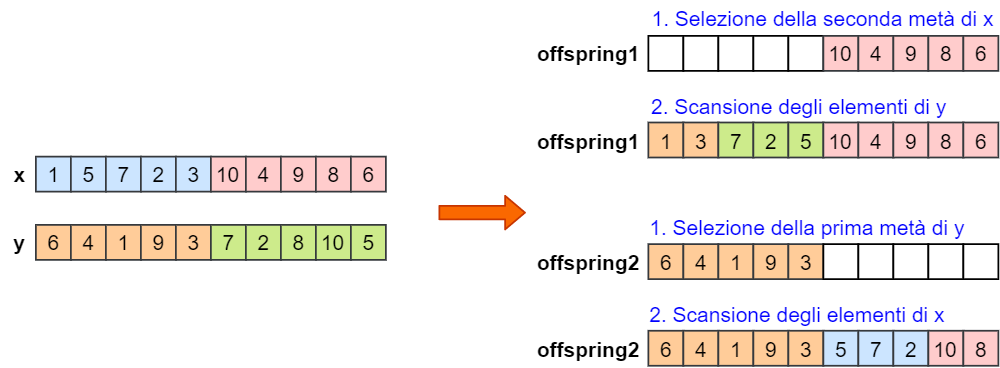
\includegraphics[scale=0.37]{Images/crossover}
  \caption{\footnotesize{Esempio di applicazione del crossover su due istanze x e y.}}
  \label{crossover}
\end{center}
\end{figure}

\begin{algorithm}[H]
\DontPrintSemicolon
\KwIn {$\mathtt{population}$= popolazione di numerosi tour generati mediante un algoritmo di costruzione\newline
$\mathtt{sum\_fitnesses}$= somma delle fitness di tutti gli individui della popolazione\newline
$\mathtt{best\_cost}$= costo della migliore soluzione attuale\newline}
\KwOut {$\mathtt{offspring1, offspring2}$= nuovo individuo generato nella popolazione}
\BlankLine
$\mathtt{n} \gets$ numero di nodi dell'istanza tsp\;
\BlankLine
$\mathtt{x=\{x_1,...,x_n\}\gets} RANDOM(population)$\;
 \BlankLine
 $\mathtt{begin} \gets RANDOM(\{1,...,n/2\})$\;
 $\mathtt{end} \gets RANDOM(\{n/2+1,...,n\})$\;  
 \BlankLine
 \For{$\mathtt{i}\gets begin$ \KwTo $end$}{
	\BlankLine
	$\mathtt{offspring[}i\mathtt{]}\gets x[end - i + begin]$\;
 }  
 
 \If{$cost(offspring) < best\_cost$}{
 	$\mathtt{best\_cost} \gets cost(offspring)$\;
 }
\caption{Mutazione}
\end{algorithm}

\begin{figure}[H]
\begin{center} 
  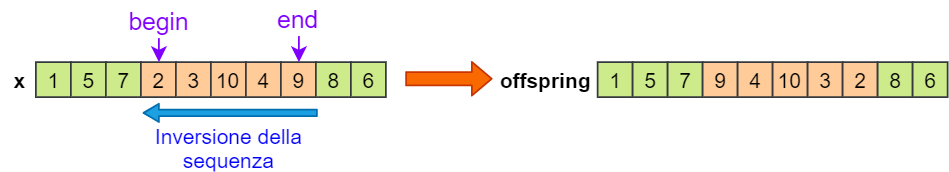
\includegraphics[scale=0.4]{Images/mutation}
  \caption{\footnotesize{Esempio di applicazione della mutazione su un'istanza x.}}
  \label{mutation}
\end{center}
\end{figure}